\documentclass{standalone}

\usepackage{tikz}

\begin{document}
	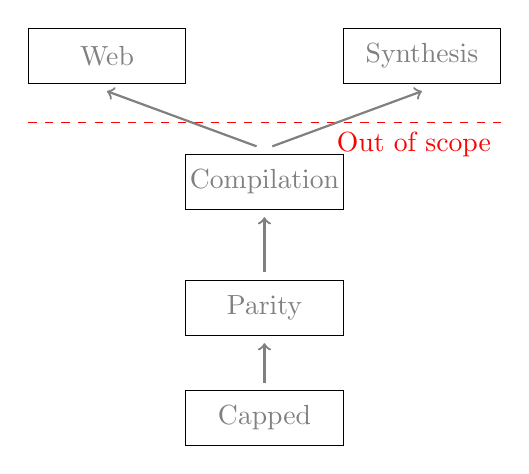
\begin{tikzpicture}
		\draw (-1, 1.4) rectangle (1, 2.1) node[midway, gray] {Capped};
		\draw [->, gray, thick] (0, 2.2) -- (0, 2.7);
		\draw (-1, 2.8) rectangle (1, 3.5) node[midway, gray] {Parity};
		\draw [->, gray, thick] (0, 3.6) -- (0, 4.3);
		\draw (-1, 4.4) rectangle (1, 5.1) node[midway, gray] {Compilation};
		\draw [red, dashed] (-3, 5.5) -- (3, 5.5) node[below left] {Out of scope};
		\draw [->, gray, thick] (-0.1, 5.2) -- (-2, 5.9);
		\draw [->, gray, thick] (0.1, 5.2) -- (2, 5.9);
		\draw (-3, 6) rectangle (-1, 6.7) node[midway, gray] {Web};
		\draw (1, 6) rectangle (3, 6.7) node[midway, gray] {Synthesis};
	\end{tikzpicture}
\end{document}
